\documentclass[10pt]{beamer}
\usetheme{Montpellier} 
\usepackage{lmodern}
\usepackage{amsmath}
\usepackage[utf8]{inputenc}
\usepackage[T1]{fontenc}
\usepackage{polski}
\usepackage[polish]{babel}
\usepackage{mathptmx}


\newcommand{\argmax}[1]{\underset{#1}{\operatorname{arg}\,\operatorname{max}}\;}
\beamertemplatenavigationsymbolsempty

\makeatletter
\setbeamertemplate{footline}
{
  \leavevmode%
  \hbox{%
  \begin{beamercolorbox}[wd=.333333\paperwidth,ht=2.25ex,dp=1ex,center]{author in head/foot}%
    \usebeamerfont{author in head/foot}\insertshortauthor~~\beamer@ifempty{\insertshortinstitute}{}{(\insertshortinstitute)}
  \end{beamercolorbox}%
  \begin{beamercolorbox}[wd=.333333\paperwidth,ht=2.25ex,dp=1ex,center]{title in head/foot}%
    \usebeamerfont{title in head/foot}\insertshorttitle
  \end{beamercolorbox}%
  \begin{beamercolorbox}[wd=.333333\paperwidth,ht=2.25ex,dp=1ex,right]{date in head/foot}%
    \usebeamerfont{date in head/foot}\insertshortdate{}\hspace*{2em}
    \insertframenumber\hspace*{2ex} 
  \end{beamercolorbox}}%
  \vskip0pt%
}
\makeatother


\author[Adam Kosiorek]{\Large Adam Kosiorek \\ \large  pod kierunkiem prof. dr hab. B. Siemiątkowskiej}
\begin{document}
\title[Rozpoznawanie obiektów 3D na podstawie danych RGBD]{\HUGE Politechnika Warszawska\\ Wydział Mechatroniki \\ \ \\ \Large Rozpoznawanie obiektów 3D na podstawie danych RGBD} 
\date{11 lutego 2014} 

\thispagestyle{empty}
\titlepage
\thispagestyle{empty}
\frame{\frametitle{Plan prezentacji}\tableofcontents}
\begin{document}

\section{Założenia i zakres pracy} 

\begin{frame}{Założenia}
  %\setcounter{framenumber}{1}
   
   Założeniem pracy jest zbadanie zagadnienia klasyfikacji metodą Bag of Words obiektów 3D na podstawie zdjęć RGBD. Zdjęcia powinny byc reprezentowane w formie chmur punktów. Ponadto zakłada się, że: \ \\
  \begin{itemize}
   \item Analizowane dane pochodzą z kamery RGBD Microsoft Kinect
   \item Implementacja algorytmu w języku C++ z wykorzystaniem bibliotek OpenCV i/lub PointCloud Library
   \item Testy aplikacji na ogólnie dostępnej, naukowej bazie danych
  \end{itemize}

\end{frame}

\begin{frame}{Zakres pracy}
  \begin{enumerate}
    \item Przegląd istniejących rozwiązań dotyczących klasyfikacji obiektów na podstawie chmur punktów
    \item Opracowanie algorytmu klasyfikacji obiektów na podstawie chmur punktów
    \item Implementacja algorytmu w języku C++ 
    \item Przeprowadzenie testów szybkości oraz skuteczności klasyfikacji 
    \item Opracowanie wniosków końcowych
  \end{enumerate}
\end{frame}


\section{Podejście Bag of Words}
\begin{frame} {Bag of Words --- wprowadzenie}
  \begin{figure}
    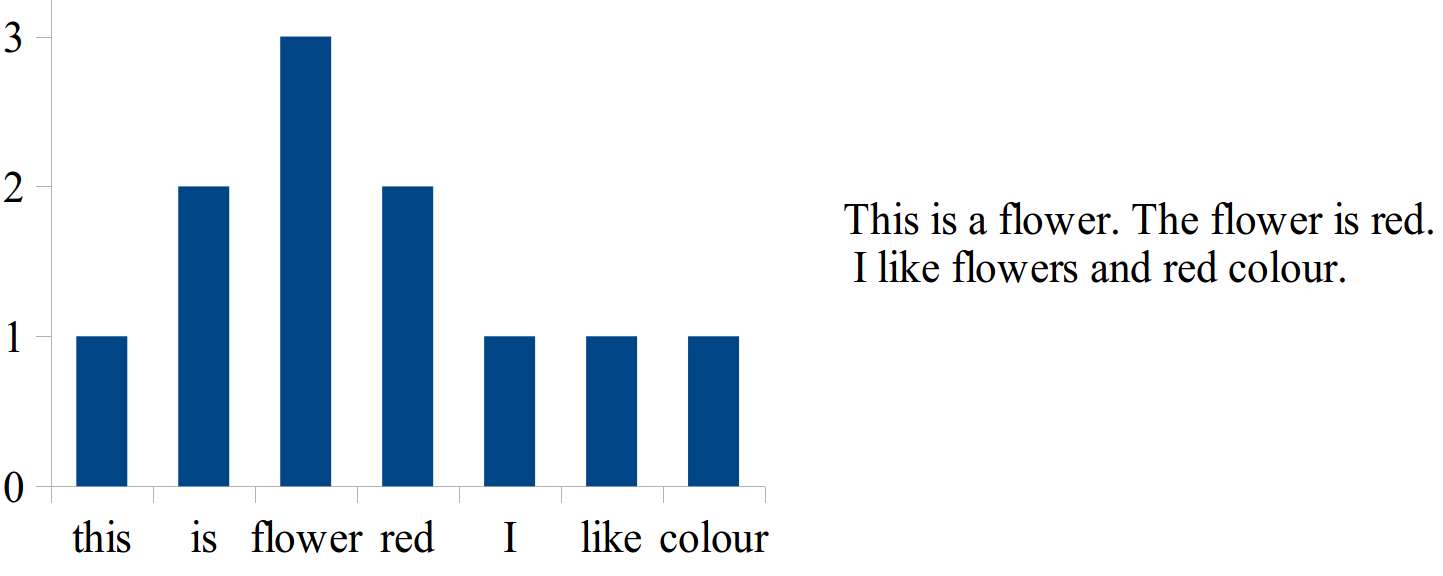
\includegraphics[scale=0.15]{../figs/bow_example}
  \end{figure}
  
  \begin{itemize}
   \item Histogram jako forma pośrednia
   \item Częstość występowania słów
   \item Usunięcie gramatyki, kolejności słów  
   \item Wymaga utworzenia słownika
   \item Reprezentacja rzadka w przypadku dużego słownika
   \item Używany m. in. do znajdowania rozkładu tematów w dokumencie (pLSA, LDA)
  \end{itemize}


\end{frame}

\begin{frame}{Bag of Words --- obrazy}	
	\begin{columns}
	
	 \begin{column}{6cm}
	 \begin{figure}
	   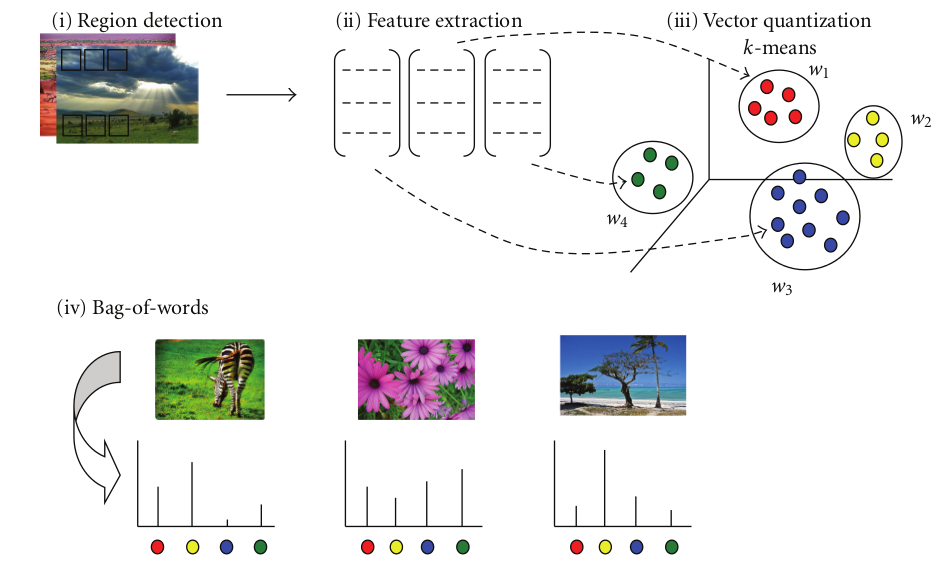
\includegraphics[scale=0.18]{../figs/tsai2012}
	   \end{figure}
	 \end{column}
	 -
	 \begin{column}{3cm}
	  \footnotesize Grafika pochodzi z C. Tsai. \textit{Bag-of-words representation in image annotation: A review. ISN Artificial Intelligence, 2012}.
	 \end{column}

	\end{columns}

	\begin{enumerate}
	 \item Wykrycie punktów charakterystycznych --- x, y, skala (SIFT, FAST)
	 \item Opisanie otoczenia wykrytych punktów --- histogram gradientów (SURF, HOG)
	 \item Budowanie słownika --- klasteryzacja (KMeans, GMM)
	 \item Klasyfikacja --- uczenie nadzorowane (SVM, Boosting)
	\end{enumerate}	
\end{frame}{}

\section{Projekt aplikacji}

\begin{frame}{Projekt aplikacji}
 \begin{figure}
	    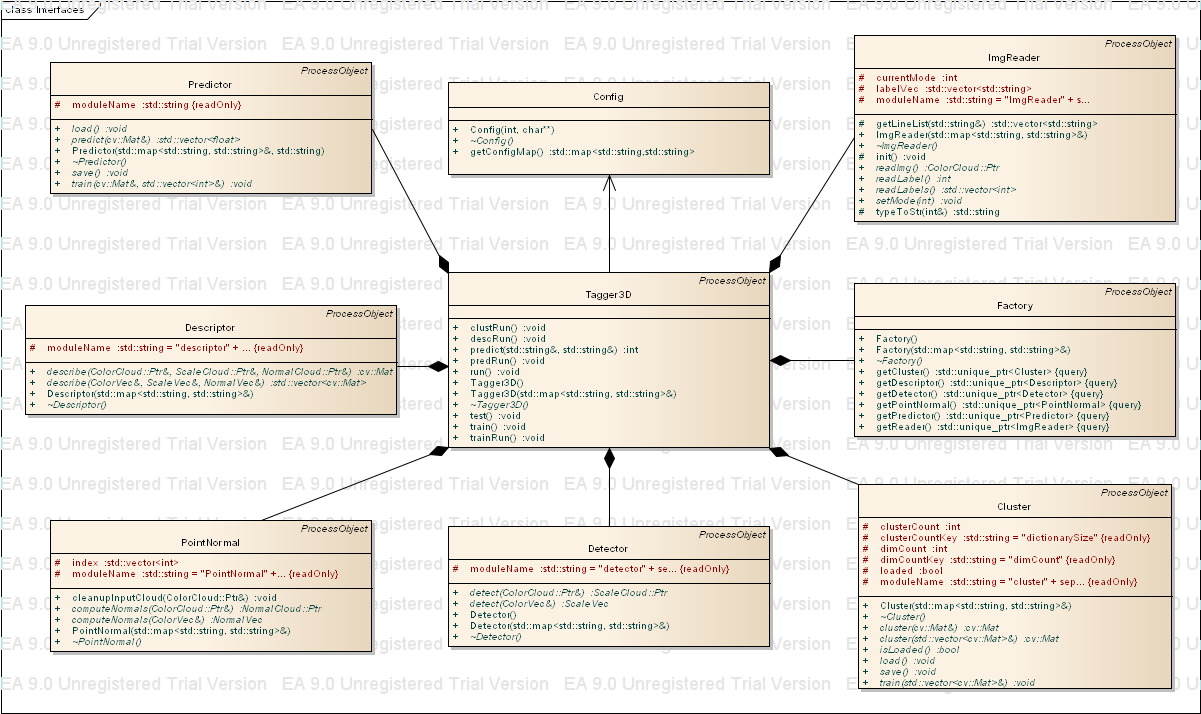
\includegraphics[width=0.9\textwidth]{../figs/class}	   
	  \end{figure}
	  \centering \footnotesize Architektura \normalsize
	  \begin{itemize}
    \item Główny obiekt --- \textit{Tagger3D}
    \item Fabryka --- tworzenie innych obiektów
    \item Konfiguracja w pliku tekstowym (Boost)
    
    \end{itemize}
 
\end{frame}


\begin{frame}{Projekt aplikacji c.d.}

	  \begin{figure}
	  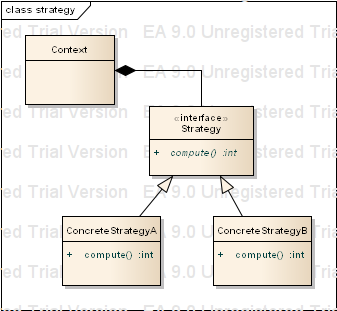
\includegraphics[width=0.5\textwidth]{../figs/strategy}	
	  \end{figure}
	  \centering \footnotesize Strategia

    \begin{itemize}
     \item Strategia --- wymiana algorytmów w sposób niewidzialny dla aplikacji
     \item Każdy etap BoW ma wydzielony interfejs (Detector, Descriptor)
     \item Obiekt IoUtils oparty o szablony obsługuje operacje wejścia/wyjścia
    \end{itemize}

\end{frame}

\section{Bazy danych}

\begin{frame}{Berkely 3D Object Dataset}
  \begin{figure}[!ht]
	    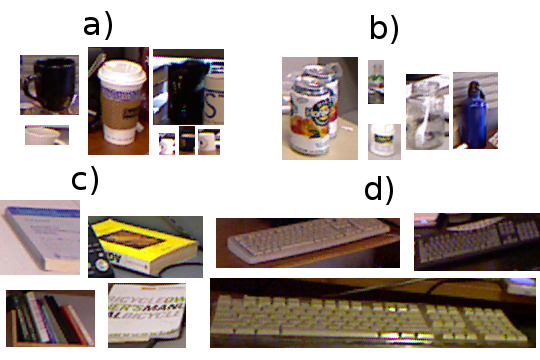
\includegraphics[scale=0.45]{../figs/b3do_objects}
	  \end{figure}
	  \centering Obiekty z B3DO. Zdjęcia w oryginalnej jakości. a)~kubek b)~butelka c)~książka d)~klawiatura
\end{frame}


\begin{frame}{Berkely 3D Object Dataset c.d.}

	  
	  \begin{itemize}
	   \item 78 kategorii obiektów
	   \item Wiele obiektów na jednym zdjęciu
	   \item Niska jakość zdjęć, wiele zdjęć niedoświetlonych, zaszumionych
	   \item Obiekty przysłonięte
	   \item Kolorowe zdjęcia i mapy głębi; Adnoacje w XML
	   \item Skrypty w Pythonie i C++ do ekstrakcji pojedynczych obiektów i podziału na kategorie.
	   \item Od 1 do 299 instancji w jednej kategorii
	   \item Losowy wybór 8 kategorii tak, żeby było~>~50 instancji w każdej kategorii
	  \end{itemize}

\end{frame}

\begin{frame}{University of Tokyo Dataset}
	\begin{figure}[!ht]
	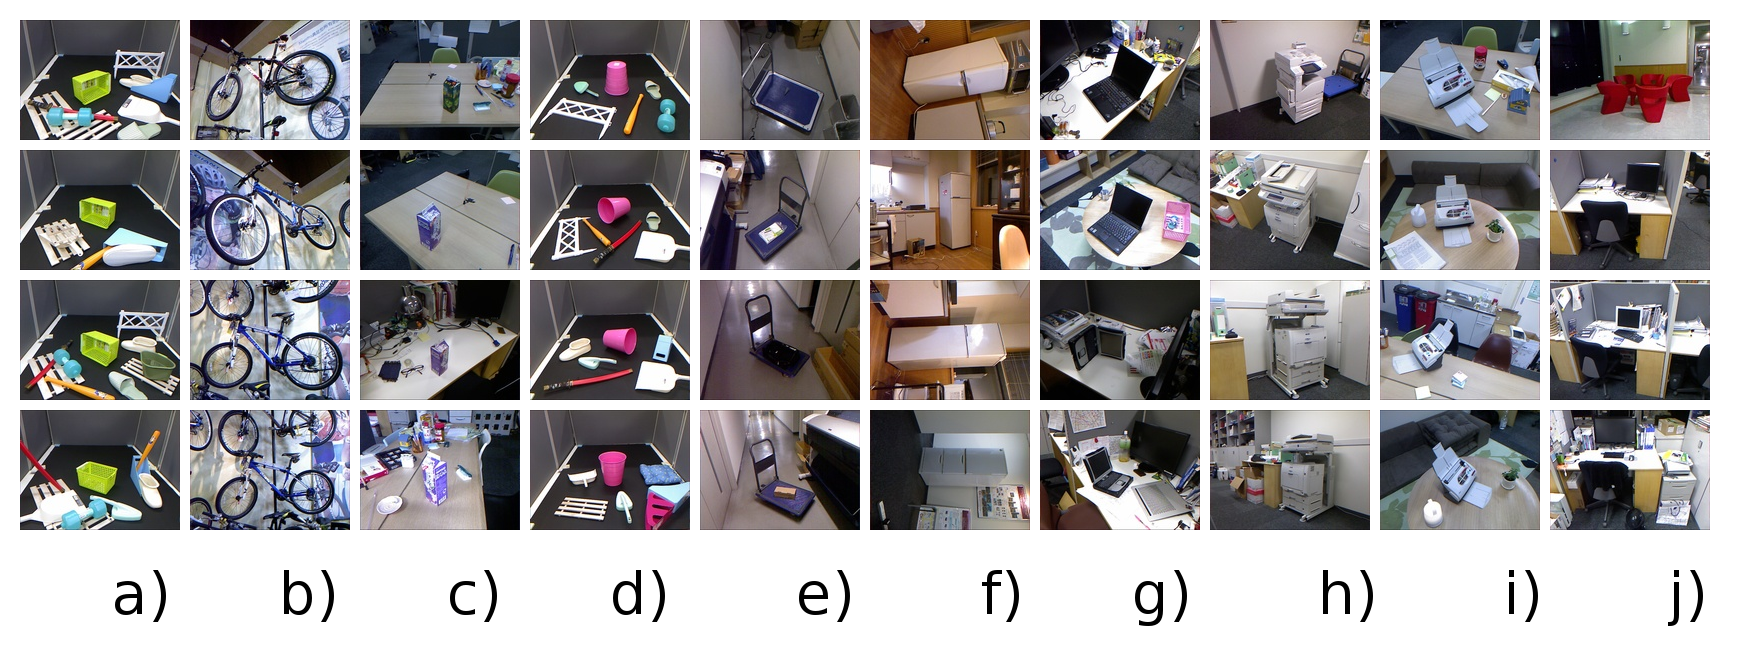
\includegraphics[scale=0.18]{../figs/tokyo_horizontal}
	\end{figure}
	\centering Baza danych Tokyo: a)~kosz b)~rower c)~pudełko d)~wiadro e)~wózek f)~lodówka g)~notebook h)~drukarka i)~skaner j)~scena
\end{frame}


\begin{frame}{University of Tokyo Dataset c.d.}
	
		\begin{columns}
		\begin{column}{5cm}
			\begin{itemize}
			\item 10 kategorii
			\item Zdjęcia dobrej jakości, dobrze naświetlone
			\item Wszystkie zdjęcia w kategorii to instancje jednego obiektu
			\end{itemize}
		\end{column}
		\begin{column}{6cm}     
			\begin{itemize}
			\item Małe różnice pomiędzy klasami obiektów:
			  \begin{itemize}
			  \item skaner i drukarka
			  \item koszyk i wiadro
			  \end{itemize}
			  \item Dane w formie: kolorowe zdjęcie + plik .csv z absolutnymi współrzędnymi wszystkich pixeli
			  \item Skrypty Python i C++ - przeksztąłcenie do chmury punktów w formacie PCD
			\end{itemize}
		\end{column}
	\end{columns}

\end{frame}

\section{Wyniki}

\begin{frame}{Porównanie algorytmów}

	\begin{columns}
	
	\begin{column}{6cm}
	\begin{table}[!ht]	
	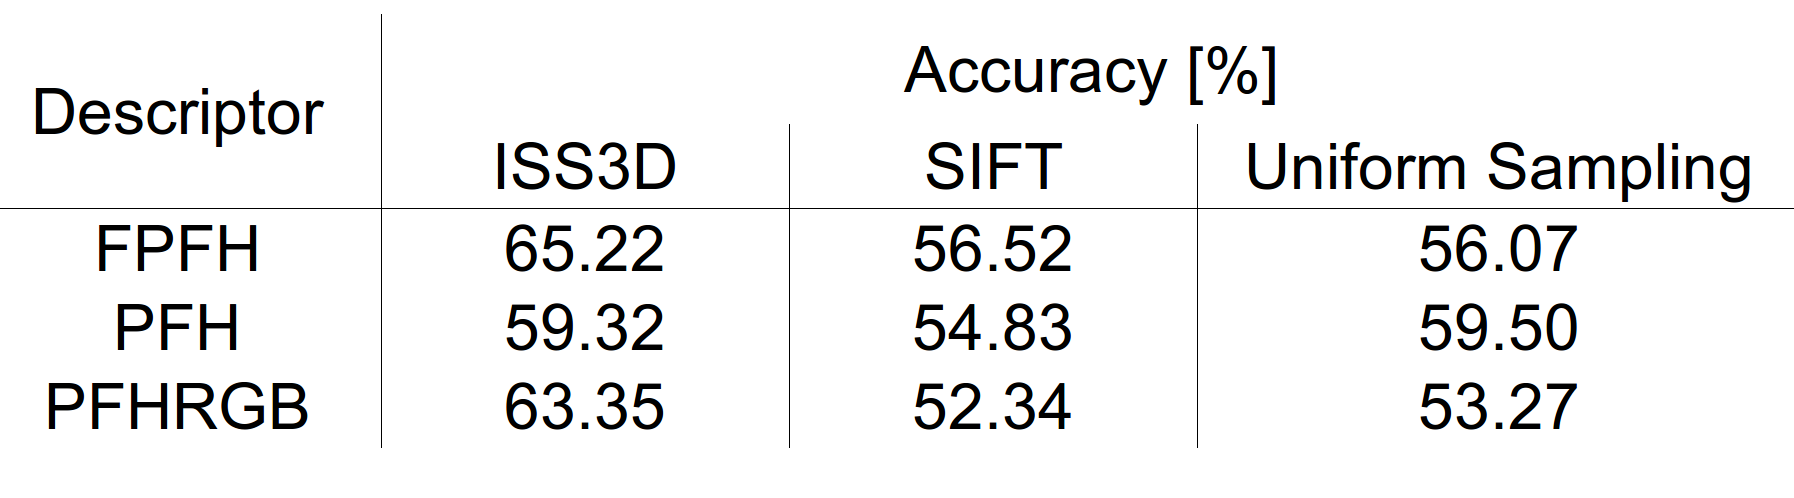
\includegraphics[scale=0.09]{../figs/desc_b3do} \\ 
	\centering
	\footnotesize Porównanie algorytmów \\
	\vspace{0.5cm}
	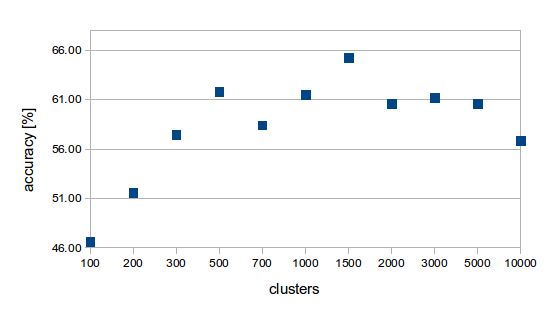
\includegraphics[scale=0.30]{../figs/clustering_centroids_b3do} \\ 
	\centering
	\footnotesize Wpływ rozmiaru słownika na skuteczność klasyfikacji
	\end{table}
	
	 \end{column}
	 
	  \begin{column}{6cm}	  
	  \begin{itemize}
	   \item Selekcja na podstawie literatury
	   \item Deskryptory PFH najlepsze w dopasowywaniu chmur punktów:
	    \begin{itemize}
	      \item PFH --- Algorytm bazowy, 125 wymiarów
	      \item FPFH --- przybliżony, 33 wymiary
	      \item PFHRGB --- uwzględnia kolor, 250 wymiarów
	    \end{itemize}
	   \item Detektory: 
	       \begin{itemize}
	      \item SIFT --- Najlepszy algorytm 2D
	      \item ISS --- Najlepsze wyniki w dopasowywaniu chmur punktów
	      \item US --- Najprostszy, równomierna siatka punktów
	    \end{itemize}
	   \item Optymalny rozmiar słownika
	  \end{itemize}

	  
	 \end{column}
	\end{columns}
	
\end{frame}

\begin{frame}{Wyniki B3DO}
		\begin{columns}
	
	 \begin{column}{8cm}
	\begin{table}[!ht]	
	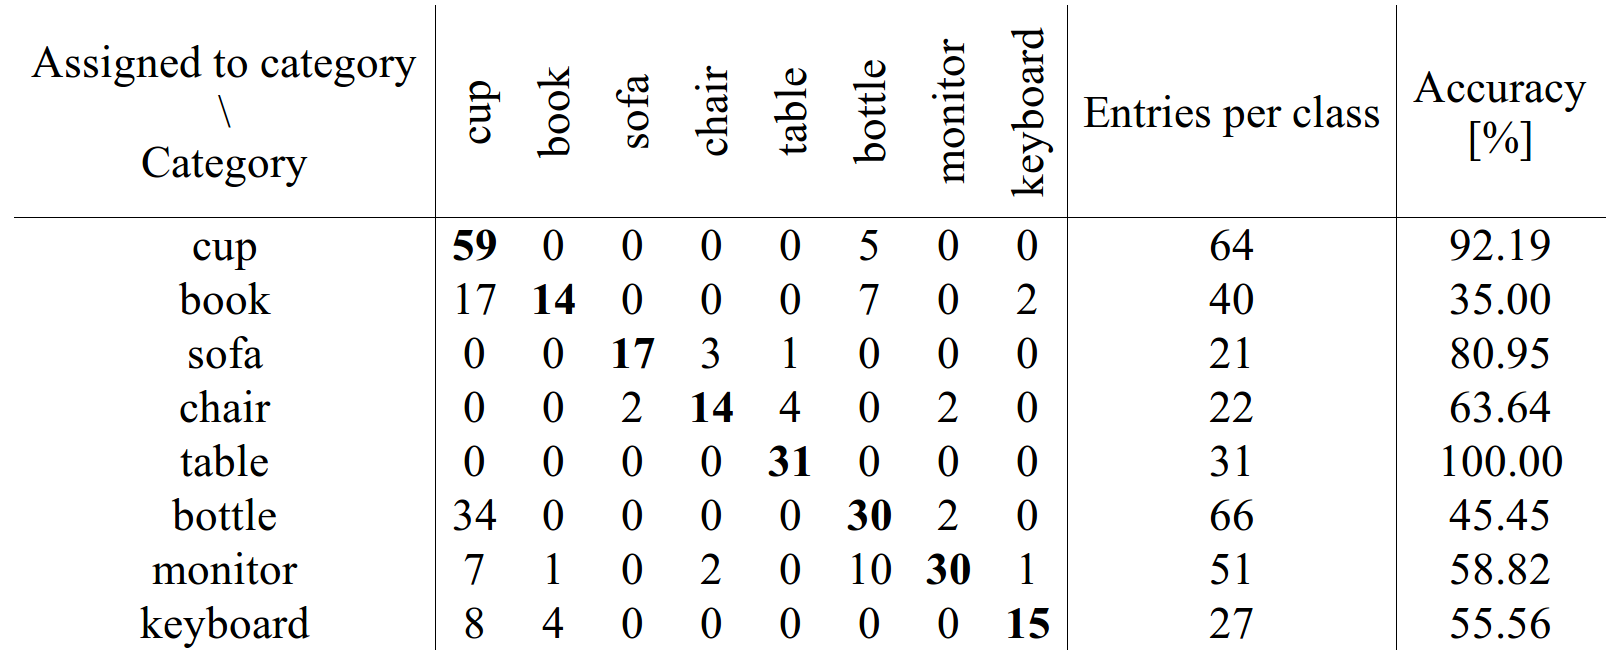
\includegraphics[scale=0.15]{../figs/b3do_conf_matrix}
	\end{table}
	 \end{column}
	  \begin{column}{2.8cm}	  
	  \footnotesize \textbf{Wynik: 65.22\%} Wyniki na bazie B3DO, detektor ISS, ekstraktor FPFH, słownik o wielkości 1500 słów
	 \end{column}
	\end{columns}		
		\begin{itemize}
	   \item Im lepiej rozdzielone kategorie obiektów, tym wyższe wyniki
	   \item Najwyższy wynik: stół, 100\%
	   \item Niskie wyniki wynikają bezpośrednio z podobieństwa między klasami: 
	   \begin{itemize}
	    \item książka, 35\%, mylona z kubkiem i butelką
	    \item butelka, 45\%, mylona z kubkiem
	   \end{itemize}
	  \end{itemize}
\end{frame}

\begin{frame}{Wyniki Tokyo}
	\begin{columns}	
	 \begin{column}{8cm}
	\begin{table}[!ht]	
	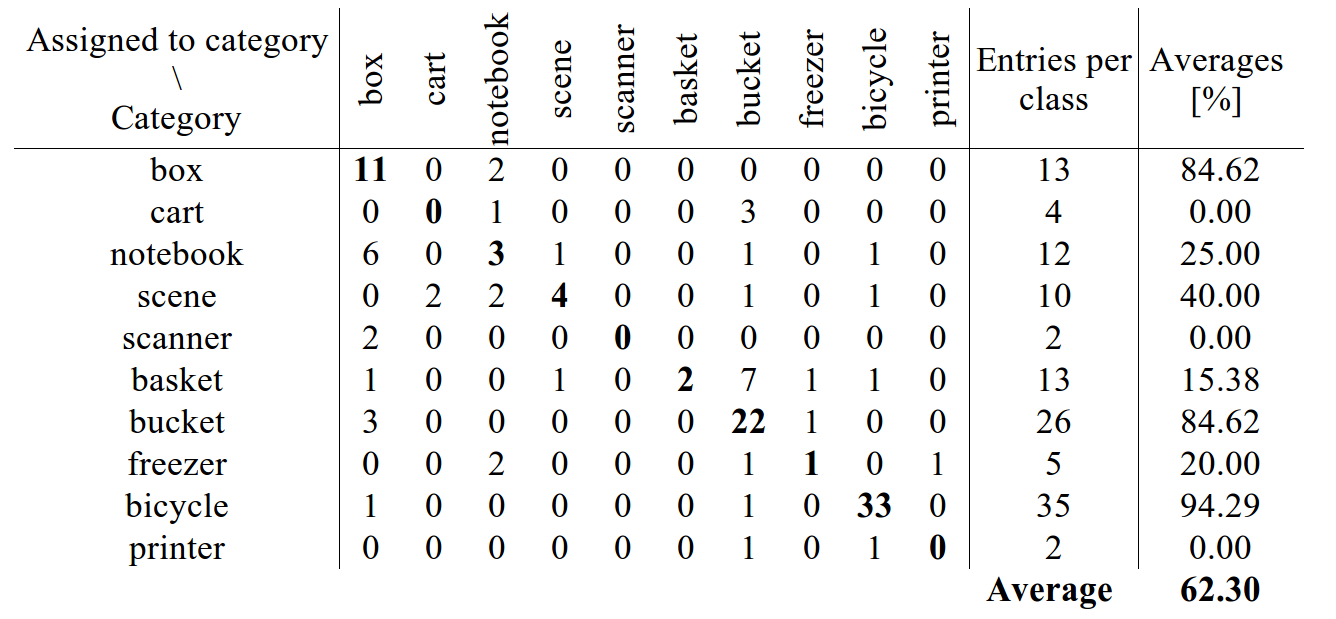
\includegraphics[scale=0.18]{../figs/tokyo_conf_matrix}
	\centering
	
	\end{table}
	
	 \end{column}
	 
	  \begin{column}{2.8cm}	  
\footnotesize \textbf{Wynik: 62.30\%} Wyniki na bazie Tokyo, detektor ISS, ekstraktor PFH, słownik o wielkości 3000 słów
	  
	 \end{column}
	\end{columns}	
	
		  \begin{itemize}
	   \item liczność w klasie \textasciitilde \ skuteczność klasyfikacji
	   \item Najwyższy wynik: rower, 94\%, największa ilośc obiektów
	   \item Najniższe wyniki : wózek, skaner, drukarka --- po 4, 2, 2 obiekty
	   \item Notebook i wiadro mylone z pudełkiem, a kosz z wiadrem
	  \end{itemize}
\end{frame}

\section{Podsumowanie}

\begin{frame}{Podsumowanie --- problemy}
 Wystąpiły następujące problemy:
	  \begin{itemize}
	    \item W zasadzie brak baz danych nadających się do zadania klasyfikacji obiektów na podstawie danych RGBD
	    \item Wymagające przetwarzanie chmur punktów ze względu na brak struktury
	    \item Najlepsze algorytmy dostępne są tylko do 2D, brak możliwości ich prostego uogólnienia do 3D
	  \end{itemize}
\end{frame}

\begin{frame}{Podsumowanie --- poprawa skuteczności i szybkości}
 Możliwości poprawy skuteczności i/lub szybkości działania aplikacji:
	    \begin{itemize}
	      \item Przeniesienie obliczeń do domeny 2D; RGB i D jako niezależne obrazy + złożenie wyników klasyfikacji
	      \item Trening klasyfikatorów na znacznie większych bazach danych
	      \item Przeniesienie obliczeń na GPU
	      \end{itemize}
\end{frame}

\begin{frame}{Podsumowanie}
	\begin{itemize}
	\item Zrealizowano wszystkie założenia projektowe
	 \item Uzyskane wyniki na bazach B3DO i Tokyo są odpowiednio $5.21$ i $6.23$ razy lepsze od kategoryzacji losowej (odpowiednio 12.5\% i 10\%)
	\end{itemize}

\end{frame}

\end{document}

